\documentclass{article}

\usepackage{graphicx}
	\graphicspath{ {images/} }


\begin{document}

\subsection{Testing strategy}

For testing purposes, we decided to use Junit to write all of our unit tests. These tests would verify the functionality of our different mathematical functions. We would need to think of and write up as many test cases as possible for different scenarios (negative numbers, large and small numbers, invalid input, etc) in order to cover all potential issues. \\

Test coverage is incredibly important in the early stages of a software project. Early and thorough testing reduces the risk of having an insurmountable amount of bugs later on. Taking this into consideration, we decided to employ a Test Driven Development strategy in which we would write unit tests before the functions were complete and imposed a rule that all valid tests must pass before any team member makes a push to our master branch. This would ensure that whenever anyone pulled from the master branch, they would not have to waste time fixing someone's bugs to work on their own task. \\

We all agree that testing each other's code is of paramount importance to the project. To not do so would lead to colossal wastes of time in tracking down myriad bugs. We made the following testing matrix which will ensure that there are no conflicts of interest in the testing. The arrow indicates who can test who - no arrow means you cannot test that person's code.

\begin{figure}[!h]
\caption{Testing matrix}
\centering
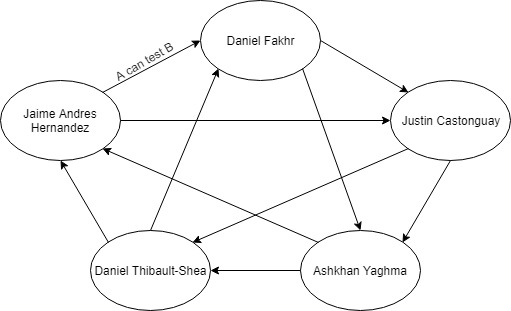
\includegraphics[width=1\textwidth]{TestingMatrix}
\end{figure}

\subsubsection{Specific testing strategies}

\end{document}